\documentclass[peer-review]{fa2026}
%\documentclass[non-peer-review]{fa2026}
% ------------------------------------

% Title, author, and affiliation
% ------------------------------------
\title{Mitigating Domain Shift in Bird Call Recognition}

\author[1]{Giotto Frean}
\author[1]{Stephen Marsland}
\correspondingauthor{stephen.marsland@vuw.ac.nz}{Stephen Marsland}

\affil[1]{School of Mathematics and Statistics, Victoria University of Wellington, New Zealand}

% Main document
% ------------------------------------
\begin{document}
\maketitle

\begin{abstract}
How severe is domain shift in bird call recognition when species distributions are held constant? We construct matched datasets with identical species distributions but different recording sources to isolate equipment and environmental effects from label distribution confounds. We observe severe, \textit{asymmetric} domain shift: models trained on diverse field recordings (AviaNZ) transfer moderately (-8.4pp), while models trained on consistent monitoring recordings (DOC) suffer catastrophic failure when deployed to diverse sources (-41.6pp). This asymmetry reveals that homogeneous training data allows models to exploit recording-specific artifacts that fail to generalize. We systematically evaluate preprocessing techniques (temporal smoothing, PCEN, Box-Cox, statistical background subtraction), domain adaptation (DANN), and augmentation strategies. Simple temporal smoothing provides the largest consistent gains, though substantial accuracy gaps remain (best cross-domain: 48.2\% vs 64\% within-domain). PCEN partially mitigates shift for consistent recordings (22\% $\to$ 41\%) but leaves performance far below within-domain accuracy. Domain adversarial training shows inconsistent, direction-dependent effects. Our central finding: \textit{domain shift in bioacoustics is fundamentally difficult—current normalization and adaptation methods provide only partial mitigation, and training data heterogeneity matters more than any preprocessing technique}. We provide a rigorous experimental methodology for isolating domain effects applicable beyond bird call recognition.
\end{abstract}

\keywords{bird call recognition, domain shift, asymmetric transfer, cross-domain evaluation, bioacoustic monitoring}

\section{Introduction}

Automated bird call recognition enables large-scale biodiversity monitoring but faces a critical deployment challenge: \textit{domain shift}. Models achieving 60-90\% accuracy on test data from the same distribution often drop to 20-40\% when applied to recordings from different equipment, locations, or environmental conditions.

A fundamental question remains unanswered: \textit{how much of observed domain shift stems from equipment and environmental differences versus species distribution mismatch?} Existing studies confound these factors—different recording sites typically have different species compositions, making it impossible to isolate the effect of recording characteristics alone.

We address this via \textbf{matched dataset construction}: two datasets with \textit{identical species distributions} but different recording sources. The DOC dataset represents Department of Conservation biodiversity monitoring recordings with consistent equipment. The AviaNZ dataset comprises diverse field recordings from varied locations across New Zealand. Both contain the same 9 species in the same proportions. This design cleanly isolates domain effects from label distribution confounds.

Our systematic evaluation of normalization techniques (temporal smoothing, PCEN, Box-Cox, statistical background subtraction), domain adaptation (DANN), and augmentation reveals three central findings:

\textbf{(1) Domain shift is severe and asymmetric.} Models trained on homogeneous recordings (DOC) suffer catastrophic cross-domain failure (-41.6pp), while models trained on heterogeneous recordings (AviaNZ) transfer moderately (-8.4pp). This asymmetry reveals that consistent training data allows exploitation of recording-specific artifacts.

\textbf{(2) Current methods provide only partial mitigation.} Simple temporal smoothing (median filtering) provides the most consistent gains, but even best-case scenarios leave accuracy far below within-domain performance (41\% vs 60\%). PCEN shows direction-dependent effectiveness. Domain adversarial training (DANN) shows inconsistent, context-dependent gains. Statistical background subtraction adds minimal benefit and can degrade performance.

\textbf{(3) Training data heterogeneity dominates preprocessing.} The \textasciitilde5$\times$ difference in domain shift magnitude between diverse and consistent training data (-8.4pp vs -41.6pp) exceeds gains from any normalization or adaptation technique we evaluate.

These findings demonstrate that domain shift in bioacoustics is fundamentally difficult. Our matched dataset methodology provides a rigorous experimental framework applicable beyond bird calls to any audio classification task where deployment conditions differ from training.

\section{Methods}

\subsection{Matched Dataset Construction}

To isolate domain shift from species distribution confounds, we created two datasets with \textit{identical species distributions}. Each contains the same proportion of 9 common New Zealand bird species: blackbird (\textit{Turdus merula}), chaffinch (\textit{Fringilla coelebs}), fantail (\textit{Rhipidura fuliginosa}), grey warbler (\textit{Gerygone igata}), kaka (\textit{Nestor meridionalis}), morepork (\textit{Ninox novaeseelandiae}), silvereye (\textit{Zosterops lateralis}), tomtit (\textit{Petroica macrocephala}), and combined tui/bellbird (\textit{Prosthemadera novaeseelandiae}/\textit{Anthornis melanura}). Both datasets contain at least 20 samples per species (~700 total).

\textbf{DOC Dataset}: Extracted from Department of Conservation biodiversity monitoring recordings.

\textbf{AviaNZ Dataset}: Field recordings collected from diverse locations across New Zealand.

Each dataset was split 75\%/25\% train/test with grouped sampling by source file to prevent data leakage. During training, the train split was further divided 80\%/20\% for training/validation. Spectrograms used 25ms Hann windows, 10ms hop, 128 mel bins (0-8kHz), 16kHz sampling rate.

\subsection{Normalization Strategies}

We compared four spectrogram normalization approaches to assess their cross-domain robustness:

\textbf{Log Transform (Baseline)}: Standard logarithmic compression:
\begin{equation}
S_{\text{log}}(f,t) = \log(S(f,t) + \epsilon)
\end{equation}
where $S(f,t)$ is the magnitude spectrogram and $\epsilon = 10^{-7}$.

\textbf{Log + Background Normalization (Proposed)}: Our strategy addresses a key limitation: standard log scaling treats all spectral energy equally, amplifying both signal and persistent background noise. We use outlier detection to distinguish bird vocalizations from background, then adaptively remove recording-specific noise floors. Applied after logarithmic compression:

\begin{enumerate}
\item Apply log transform: $S_{\text{log}}(f,t) = \log(S(f,t) + \epsilon)$
\item \textbf{Temporal smoothing}: Apply 5-frame median filter along time axis to reduce transient artifacts while preserving signal structure
\item \textbf{Background estimation} per frequency band:
   \begin{itemize}
   \item Identify bottom 10\% of time frames by intensity (quietest moments, likely pure background)
   \item Compute mean $\mu_0(f)$ and standard deviation $\sigma_0(f)$ from these frames
   \item Z-score normalize: $z(f,t) = (S_{\text{log}}(f,t) - \mu_0(f)) / \sigma_0(f)$
   \item Identify outliers: pixels with $z(f,t) > 4$ (likely bird calls, >4$\sigma$ from background)
   \item Create background estimate: replace outlier values with typical background levels randomly sampled from non-outliers, then convert back to log scale: $\text{BG}(f,t)$
   \end{itemize}
\item \textbf{Subtract} background estimate: $S_{\text{norm}}(f,t) = S_{\text{log}}(f,t) - \text{BG}(f,t)$
\end{enumerate}

This sets persistent background pixels near zero while preserving transient acoustic events, adaptively removing equipment artifacts and recording-specific noise floors. Unlike PCEN's exponential smoothing with fixed time constants, our approach explicitly models the signal-background distinction using statistical outlier detection. The method requires no learned parameters and adds negligible computational overhead (<1\% of spectrogram computation time).

We also test a variant \textbf{without the median filter} (Log+normalize\_no\_median) to assess the contribution of temporal smoothing.

\textbf{PCEN}: Per-Channel Energy Normalization applies adaptive gain control to normalize each frequency band:
\begin{equation}
\text{PCEN}(f,t) = \left(\frac{S(f,t)}{(M(f,t) + \epsilon)^{\alpha}} + \delta\right)^r - \delta^r
\end{equation}
where $M(f,t)$ is a smooth temporal average computed via IIR filtering. We use standard parameters from speech recognition: $\alpha=0.8$, $\delta=10$, $r=0.25$, time constant 60ms.

\textbf{Box-Cox}: Power transformation for distribution normalization, commonly used for variance stabilization.

\subsection{Model Architecture and Training}

We use transfer learning with a BirdClef-pretrained RegNetY-008 CNN\cite{radosavovic2020designing}, replacing the final classification layer for 9 species. The pretrained model was trained on BirdClef 2023 data covering >260 species, providing strong feature representations for bird vocalizations.

Training uses AdamW optimizer with differential learning rates (lr $10^{-4}$ for backbone, $10^{-3}$ for classifier head), batch size 16, cosine annealing schedule, up to 100 epochs with early stopping (patience=15 on validation loss), and mixup augmentation ($\alpha = 0.25$) to improve generalization. We do not freeze the backbone, allowing full fine-tuning to adapt to our target species and recording conditions.

\subsection{Experimental Design}

We conduct systematic cross-domain evaluation combining training sources, normalization strategies, and domain adaptation techniques:

\begin{itemize}
\item \textbf{Training scenarios}: (1) Train on AviaNZ, test on both AviaNZ and DOC; (2) Train on DOC, test on both DOC and AviaNZ
\item \textbf{Evaluation}: Within-domain accuracy (train and test from same source) and cross-domain accuracy (test on opposite source)
\item \textbf{Normalization methods}: Log baseline, Log+normalize, Log+normalize\_no\_median, PCEN, Box-Cox
\item \textbf{Domain adaptation}: Domain Adversarial Neural Networks (DANN) with gradient reversal layer, tested with Log+normalize preprocessing
\item \textbf{Noise augmentation}: Additive ambient noise at varying intensities (0.0-1.0 ratio) and variety (1-1000 noise sources), applied during training with Log baseline
\end{itemize}

All experiments use identical train/val/test splits to ensure fair comparison. Implementation in PyTorch 2.0; each configuration run once (100 epochs with early stopping).

\begin{figure}[t]
\centering
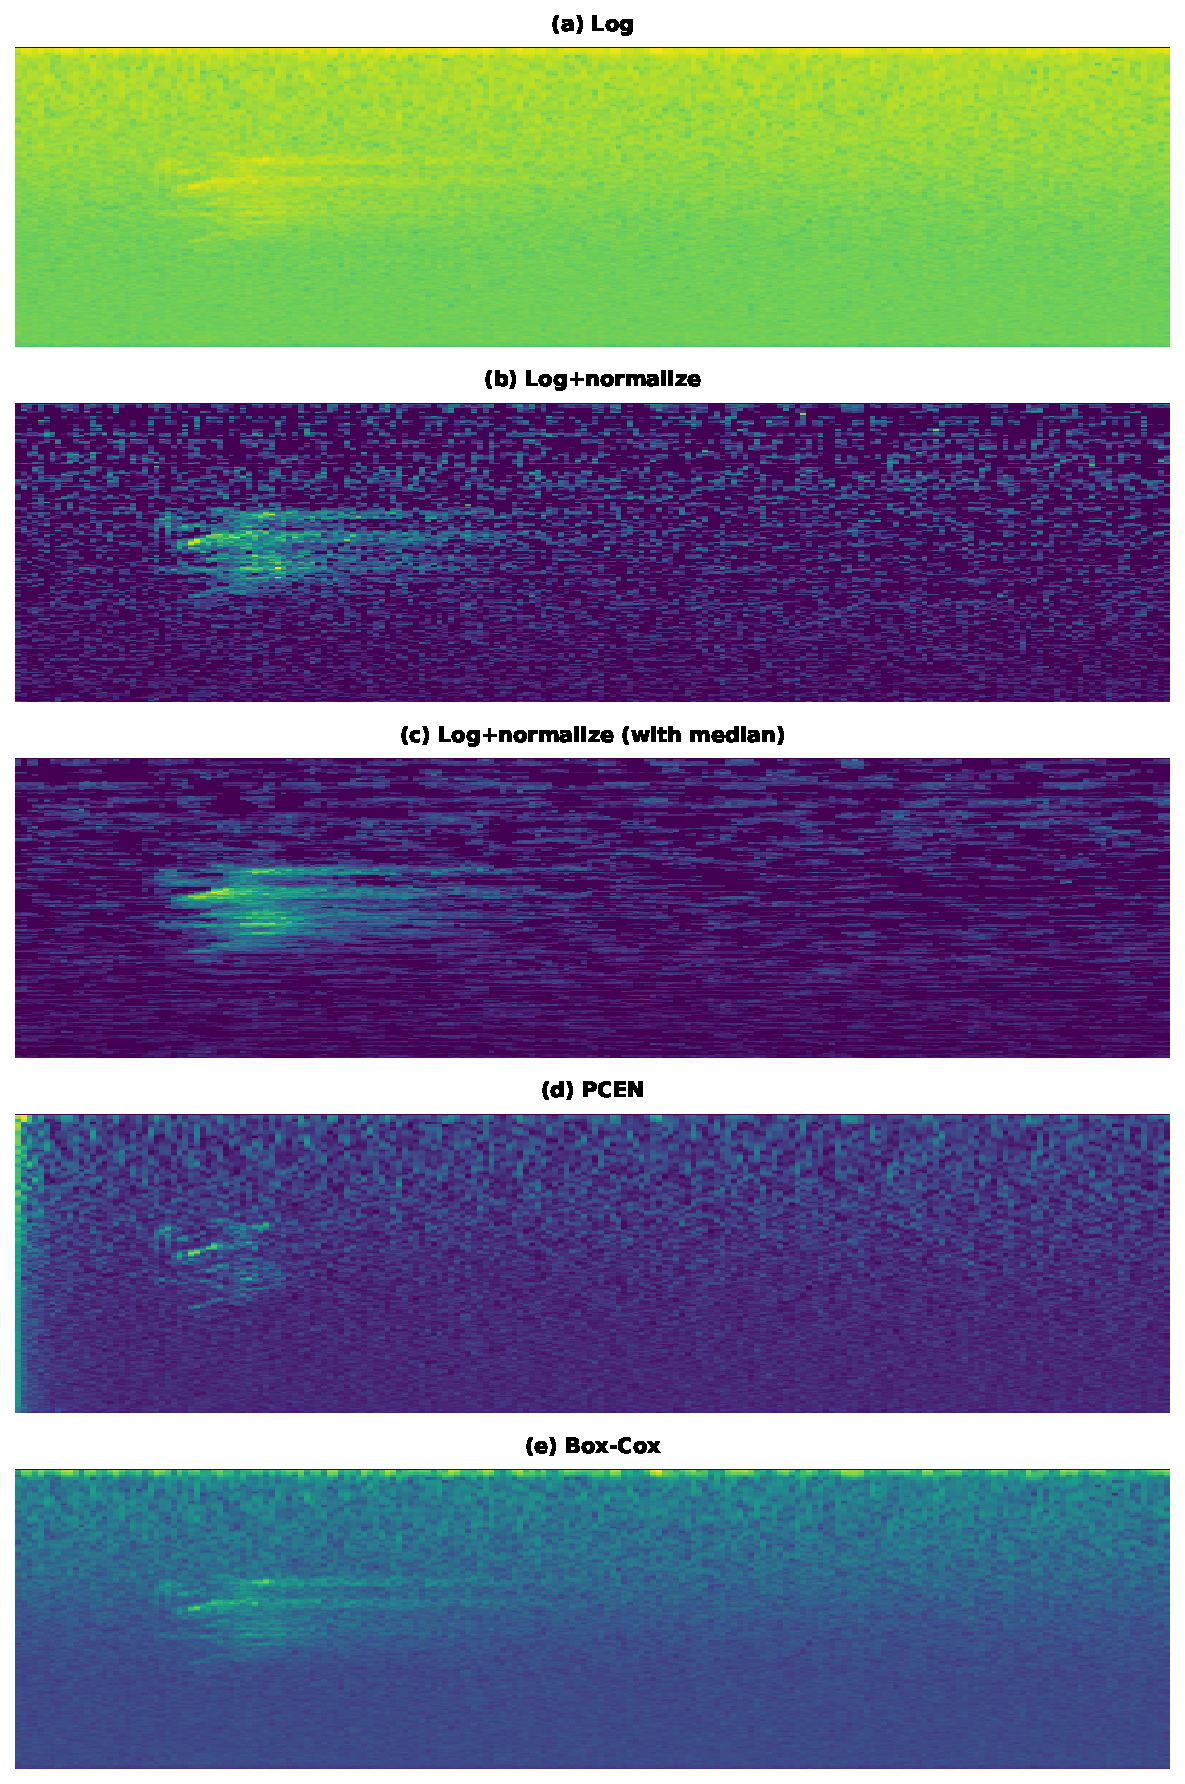
\includegraphics[width=\columnwidth]{figures/spectrogram_comparison.pdf}
\caption{Spectrogram comparison for a tui vocalization from different domains: (a) Log baseline shows persistent background noise floor characteristic of the recording equipment; (b) Log+normalize adaptively removes equipment-specific background while preserving vocalization structure; (c) PCEN applies uniform smoothing without background removal. Our method targets domain-specific artifacts.}
\label{fig:spectrograms}
\end{figure}

\section{Results}

\begin{table}[t]
\centering
\small
\caption{Cross-domain performance comparison. All values are exact-match accuracy.}
\label{tab:results}
\begin{tabular}{@{}lcccc@{}}
\hline
Method & Train & In-Dom & Cross & Shift \\
\hline
\multicolumn{5}{c}{\textit{Train on AviaNZ, test on both}} \\
\hline
Log (baseline) & AviaNZ & 52.4 & 44.0 & \textbf{-8.4} \\
Log+median\_only & AviaNZ & 49.4 & 45.2 & -4.2 \\
Log+norm\_no\_median & AviaNZ & 42.2 & 38.6 & -3.6 \\
Log+norm (full) & AviaNZ & 50.6 & 43.4 & \textbf{-7.2} \\
PCEN & AviaNZ & 45.2 & 36.7 & -8.5 \\
Box-Cox & AviaNZ & 49.4 & 36.7 & -12.7 \\
DANN+Log+norm & AviaNZ & 53.6 & 48.2 & -5.4 \\
\hline
\multicolumn{5}{c}{\textit{Train on DOC, test on both}} \\
\hline
Log (baseline) & DOC & 63.9 & 22.3 & \textbf{-41.6} \\
Log+median\_only & DOC & 59.6 & 36.7 & -22.9 \\
Log+norm\_no\_median & DOC & 53.6 & 34.9 & -18.7 \\
Log+norm (full) & DOC & 60.2 & 38.0 & \textbf{-22.2} \\
PCEN & DOC & 60.2 & 41.0 & -19.3 \\
Box-Cox & DOC & 62.0 & 27.1 & -34.9 \\
DANN+Log+norm & DOC & 57.2 & 36.1 & -21.1 \\
\hline
\end{tabular}
\end{table}

\subsection{Baseline Domain Shift Magnitude}

Using standard log scaling (Table~\ref{tab:results}), we observe severe asymmetric domain shift. Training on AviaNZ achieves 52.4\% within-domain, dropping to 44.0\% cross-domain (-8.4pp). Training on DOC achieves 63.9\% within-domain but only 22.3\% cross-domain (-41.6pp)—a 5$\times$ difference in shift magnitude. This asymmetry reveals that homogeneous training data allows models to exploit recording-specific artifacts (equipment signatures, noise patterns) that fail catastrophically when deployed elsewhere, while heterogeneous training forces reliance on generalizable features.

\subsection{Impact of Background Normalization}

Our proposed normalization (Log+norm) shows mixed and limited results:
\begin{itemize}
\item \textbf{AviaNZ training}: Cross-domain accuracy drops slightly from 44.0\% to 43.4\% (-0.6pp), with the generalization gap improving modestly (from -8.4pp to -7.2pp). Within-domain performance also drops: 52.4\% $\to$ 50.6\% (-1.8pp).
\item \textbf{DOC training}: Cross-domain shows meaningful improvement: 22.3\% $\to$ 38.0\% (+15.7pp). However, within-domain performance decreases: 63.9\% $\to$ 60.2\% (-3.7pp). The generalization gap improves from -41.6pp to -22.2pp, but performance remains far below within-domain accuracy.
\end{itemize}

The benefits are context-dependent and always partial. The method trades some within-domain accuracy for improved cross-domain robustness, but even best-case scenarios leave substantial accuracy gaps. The asymmetric gains suggest the approach is most effective when training data has consistent noise characteristics (DOC) but provides minimal benefit when training data is already diverse (AviaNZ).

\subsection{Decomposing Normalization Components}

Ablation reveals that \textbf{median filtering alone} provides nearly all observed cross-domain benefits. For AviaNZ training, median-only (45.2\% cross-domain) outperforms the full method (43.4\%). For DOC training, median-only captures 87\% of the full method's improvement (14.4pp of 15.7pp gain over baseline). Background subtraction without median filtering severely degrades accuracy (AviaNZ: 42.2\%/38.6\%; DOC: 53.6\%/34.9\%), and adding it to median filtering provides minimal benefit (+1.3pp for DOC) or harms performance (-1.8pp for AviaNZ). The median filter's effectiveness stems from removing temporal artifacts while preserving signal structure.

\subsection{PCEN Performance}

PCEN shows direction-dependent effectiveness. For AviaNZ training, it achieves similar shift to baseline (-8.5pp vs -8.4pp) with lower absolute accuracy. For DOC training, PCEN provides the best cross-domain performance (41.0\%, +18.7pp over baseline), likely due to effective normalization of consistent recording artifacts, though still far below within-domain accuracy (60.2\%).

\subsection{Box-Cox Transformation Underperforms}

Box-Cox transformation consistently underperforms across cross-domain conditions. For AviaNZ training: 49.4\% within-domain and 36.7\% cross-domain (-12.7pp shift), similar to PCEN but worse than baseline. For DOC-trained models: 62.0\% within-domain and 27.1\% cross-domain (-34.9pp shift), better than baseline (22.3\%) but substantially worse than PCEN (41.0\%) or our method (38.0\%). The transformations may normalize distribution shapes but fail to remove domain-specific spectral patterns as effectively as other approaches.

\subsection{Domain Adversarial Neural Networks}

DANN shows inconsistent, direction-dependent effects. For AviaNZ training, DANN achieves the best cross-domain performance (48.2\%, +4.8pp over Log+norm). For DOC training, DANN degrades performance (36.1\% vs 38.0\% baseline, -1.9pp). This suggests domain adversarial training requires source diversity to learn invariant features; homogeneous training allows spurious pattern learning that interferes with generalization. The modest gains and risk of degradation make DANN unreliable compared to simpler preprocessing approaches.

\section{Discussion}

\subsection{Key Findings}

\textbf{(1) Severe asymmetric shift}: Training on homogeneous recordings (DOC) enables artifact exploitation, achieving high within-domain accuracy (63.9\%) but catastrophic cross-domain failure (22.3\%, -41.6pp). Training on diverse recordings (AviaNZ) forces generalizable features, sacrificing within-domain accuracy (52.4\%) for robust transfer (44.0\%, -8.4pp).

\textbf{(2) Median filtering is most effective}: Simple 5-frame temporal smoothing provides 87\% of observed improvements with negligible overhead, outperforming complex statistical background modeling.

\textbf{(3) Methods provide partial mitigation}: PCEN achieves best DOC cross-domain performance (41.0\%), DANN best for AviaNZ (48.2\%), but both remain far below within-domain accuracy. Training data heterogeneity (33pp shift difference) exceeds preprocessing gains (5-19pp).







\subsection{Training Data Heterogeneity and Cross-Domain Transfer}

The substantial difference in transfer difficulty (DOC$\to$AviaNZ: -41.6pp versus AviaNZ$\to$DOC: -8.4pp) suggests that training on diverse recordings produces more robust features than training on consistent recordings, even when consistent training achieves higher within-domain accuracy (63.9\% vs 52.4\%).

For conservation monitoring programs, this suggests that including heterogeneous recordings in training data may improve cross-deployment robustness compared to limiting data to a single recording source, though the optimal balance requires further study across multiple sites and species sets. Our results come from comparing two specific datasets—one with diverse sources (AviaNZ) and one with consistent sources (DOC)—not from a controlled interpolation of diversity levels.

\textbf{Important limitation}: We cannot cleanly separate the effect of "diversity" from other confounds. The AviaNZ and DOC datasets differ in:
\begin{itemize}
\item Source diversity (by design)
\item Recording equipment and settings
\item Geographic distribution
\item Recording practices and quality control
\item Possibly label noise or annotation conventions
\end{itemize}

The asymmetric transfer could stem from any combination of these factors, not solely "diversity" as an abstract property. Controlled experiments varying diversity while holding other factors constant would be needed to isolate this effect definitively.


\subsection{Noise Augmentation}

Noise augmentation (tested at intensities 0.0-1.0) degraded performance across all conditions. Moderate noise (0.25-0.5) reduced accuracy by 2-3pp; high noise (1.0) caused catastrophic failure. Varying noise source diversity (1-1000 types) provided no benefit. This suggests our implementation or architecture does not effectively leverage noisy training data.

\subsection{Practical Recommendations}

For similar bioacoustic classification tasks: (1) Apply 5-frame median filtering for consistent gains with negligible cost; (2) For consistent recordings, PCEN provides best cross-domain performance; (3) For diverse recordings, DANN shows modest improvements but added complexity; (4) Prioritize training data diversity over volume from single sources; (5) Avoid noise augmentation unless validated on held-out cross-domain data; (6) Statistical background subtraction provides minimal benefit. Empirical validation on specific datasets is essential—method effectiveness varies substantially by training data characteristics.

\subsection{Limitations}

Single runs per configuration limit statistical robustness. Results are specific to 9 New Zealand species with two recording sources; generalization to larger species sets, other regions, or different equipment requires validation. Aggregate accuracy obscures per-class patterns and potential annotation inconsistencies. We infer feature learning from accuracy patterns without direct representation analysis. The AviaNZ/DOC datasets differ in multiple dimensions beyond source diversity, preventing clean attribution of observed asymmetry to any single factor.

\section{Conclusion}

We investigate domain shift in bird call recognition by constructing matched datasets with identical species distributions but different recording sources. This methodology cleanly isolates equipment and environmental effects from label distribution confounds—an approach applicable to any bioacoustic or audio classification task where deployment conditions differ from training.

Our central empirical finding is \textbf{severe, asymmetric domain shift}: models trained on homogeneous recordings (DOC) suffer catastrophic cross-domain failure (-41.6pp), while models trained on heterogeneous recordings (AviaNZ) transfer moderately (-8.4pp). This asymmetry reveals that consistent training data allows models to exploit recording-specific artifacts (equipment signatures, background patterns) that completely fail to generalize. High within-domain validation accuracy (63.9\% for DOC) does not predict cross-domain robustness (22.3\%)—a critical finding for deployment planning.

We systematically evaluate preprocessing techniques (temporal smoothing, PCEN, Box-Cox, statistical background subtraction), domain adaptation (DANN), and augmentation. Simple temporal smoothing via median filtering provides the most consistent improvements across training scenarios. PCEN shows direction-dependent effectiveness, partially mitigating shift for consistent recordings (22\% $\to$ 41\%) but leaving performance far below within-domain accuracy. Domain adversarial training shows inconsistent, modest gains in favorable conditions (+4.8pp) but can degrade performance in unfavorable conditions (-1.9pp). Our proposed statistical background subtraction adds minimal benefit over median filtering and sometimes harms performance.

\textbf{Critical insight}: Current normalization and adaptation methods provide only partial mitigation of domain shift. Even best-case scenarios leave accuracy substantially below within-domain performance (48\% cross-domain vs 64\% within-domain using DANN with AviaNZ training). The magnitude of shift reduction from training data characteristics (\textasciitilde33pp difference between diverse vs consistent training) exceeds gains from any preprocessing or adaptation technique we evaluate (\textasciitilde5-19pp improvements over baseline).

These findings demonstrate that domain shift in bioacoustics is fundamentally difficult and not solved by current techniques. For practitioners: empirical validation on held-out cross-domain data is essential. Temporal smoothing (median filtering) provides consistent modest improvements with minimal complexity. Training data heterogeneity appears to matter more than preprocessing choices, though this observation requires validation across controlled diversity levels and multiple deployment scenarios.

Our matched dataset methodology provides a rigorous experimental framework for isolating and quantifying domain effects, enabling more reliable evaluation of domain adaptation techniques and deployment robustness in biodiversity monitoring systems.

\section{Acknowledgments}
We thank the New Zealand Department of Conservation for providing access to biodiversity monitoring recordings, and the AviaNZ community for field recording contributions. This research was supported by Victoria University of Wellington.

% Bibliography placeholder - add your .bib file
%\bibliographystyle{plain}
%\bibliography{references}

\end{document}